\documentclass[tufte-handout]{standalone}
\usepackage{mathpazo} % Sets Palatino as the main font
\usepackage{tikz}
\usetikzlibrary{3d, angles, quotes, calc, backgrounds}
\usetikzlibrary{decorations.markings}

\definecolor{darkslategray}{rgb}{0.18, 0.31, 0.31}

\tikzstyle{devel} = [rectangle, rounded corners, minimum width=3cm, minimum height=1cm,text centered, draw=darkslategray!50, fill=darkslategray!0]
\tikzstyle{process} = [rectangle, rounded corners, minimum width=3cm, minimum height=1cm, text centered, draw=darkslategray!30, fill=darkslategray!30]
\tikzstyle{steps} = [rectangle, rounded corners, minimum width=3cm, minimum height=1cm, text centered, very thick, draw=darkslategray!90, fill=darkslategray!30]
\tikzstyle{decision} = [rectangle, rounded corners, minimum width=3cm, minimum height=1cm, text centered, draw=orange!30, fill=orange!30]
\tikzstyle{arrow} = [thick,->,>=stealth]
\tikzstyle{line} = [thick,-,>=stealth]


\begin{document}

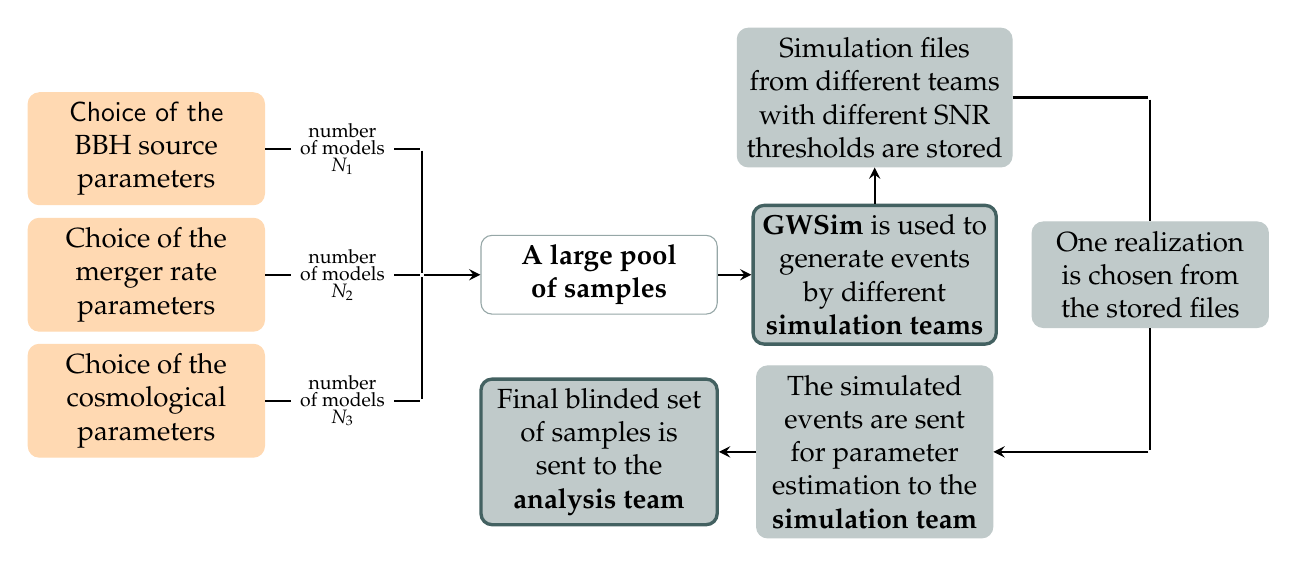
\begin{tikzpicture}[node distance=1.5cm, every node/.style={fill=white}, align=center]

% Nodes
\node (start1) [decision] {\sffamily Choice of the \\BBH source \\parameters};

%\node (start2) [decision, below of=start1, yshift=0.25cm] {Choice of \\waveforms};

\node (start3) [decision, below of=start1, yshift=-0.1cm] {Choice of the \\merger rate \\ parameters};

%\node (start4) [decision, below of=start3, yshift=-0.1cm] {Choice of the \\GW host galaxy \\from a catalog};

\node (start5) [decision, below of=start3, yshift=-0.1cm] {Choice of the \\cosmological \\parameters};

\node (central) [devel, right of=start3, xshift=4.25cm] {\bf{A large pool} \\\bf{of samples}};

\node (right1) [steps, right of=central, xshift=2cm] {\texttt{\bf GWSim} is used to\\ generate events \\by different \\ \bf simulation teams};

\node (right2) [process, right of=right1, xshift=2cm] {One realization \\is chosen from \\the stored files};

\node (up) [process, above of=right1, yshift=0.75cm] {Simulation files\\ from different teams\\ with different SNR\\ thresholds are stored};

\node (down) [process, below of=right1, yshift=-0.75cm] {The simulated \\events are sent \\for parameter\\ estimation to the \\\bf simulation team};

\node (leftofdown2) [steps, left of=down, xshift=-2cm] {Final blinded set \\of samples is \\sent to the \\\bf analysis team};

\node (anchor1) [inner sep=0pt, right of=start1, xshift=2cm]{};
%\node (anchor2) [right of=start2, xshift=2cm]{};
\node (anchor3) [inner sep=0pt, right of=start3, xshift=2cm]{};
\node (anchor5) [inner sep=0pt, right of=start5, xshift=2cm]{};

\node (anchorCentral) [inner sep=0pt, right of=start3, xshift=2cm]{};


\draw [arrow] (anchorCentral)--(central);
% Arrows
\draw [line] (start3) -- node[right of=start3, xshift=-1.5cm, execute at begin node = \setlength{\baselineskip}{0.42em}] {\scriptsize{number} \\\scriptsize{of models} \\\scriptsize{$N_2$}} (anchor3);



\draw[line] (start1)  -- node[right of=start1, xshift=-1.5cm, execute at begin node = \setlength{\baselineskip}{0.42em}] {\scriptsize{number} \\\scriptsize{of models} \\\scriptsize{$N_1$}} (anchor1);
\draw [line] (anchor1) -- (anchorCentral);
\draw [line] (start5) -- node[right of=start5, xshift=-1.5cm, execute at begin node = \setlength{\baselineskip}{0.42em}] {\scriptsize{number} \\\scriptsize{of models} \\\scriptsize{$N_3$}} (anchor5);

\draw [line] (anchor5) -- (anchorCentral);

\draw [arrow] (central) -- (right1);
%\draw [arrow] (right1) -- (right2);
\draw [arrow] (right1) -- (up);

\node (upright)  [inner sep=0pt, above of=right2, yshift=0.75cm]{};
\node (downright)  [inner sep=0pt, below of=right2, yshift=-0.75cm]{};
\draw [line] (up) -- (upright);
\draw [line] (upright) -- (right2);
\draw [line] (right2) -- (downright);
\draw [arrow] (downright) -- (down);
\draw [arrow] (down) -- (leftofdown2);

    
\end{tikzpicture}
\end{document}

